\documentclass[12pt,oneside,letterpaper]{article}
\usepackage[margin=1in]{geometry}
\usepackage{listings}
\lstset{language=C++,
                basicstyle=\ttfamily,
                keywordstyle=\color{blue}\ttfamily,
                stringstyle=\color{red}\ttfamily,
                commentstyle=\color{green}\ttfamily,
                morecomment=[l][\color{magenta}]{\#}
}
\usepackage{color}
\usepackage{graphicx}
\usepackage{hyperref}
\usepackage{amsmath}
\usepackage{amsfonts}
\title{OpenGM Demo}
\author{Vikas Dhiman}
\begin{document}
\maketitle
\section{Installation}
Please follow \href{http://www.andres.sc/publications/opengm-2.0.2-beta-manual.pdf}{OpenGM manual} for installation.

If you are facing problems OpenGM installation, we have a virtual machine setup
which I'll post on piazza. 

\section{Introduction}
Using probablistic graphical models consists of two main steps. 
\begin{enumerate}
  \item Modeling
  \item Inference
\end{enumerate}

However, when we are using a standard library like OpenGM, we have few more steps that need to be considered.
\begin{enumerate}
  \item Modeling
  \begin{enumerate}
    \item Adapting the model to OpenGM compatible format
    \item Coding the model
  \end{enumerate}
  \item Inference
    \begin{enumerate}
      \item Identifying the problem to OpenGM compatible format
      \item Coding and running the model
      \item Mapping back the solution from OpenGM to our original problem
    \end{enumerate}
\end{enumerate}

OpenGM is vast library with plethora of features. We can't cover all features
in today's demo, but hopefully this demo will give you a headstart with the
library. The official manual starts with abstract definitions followed by
examples. We will try the opposite methodology, starting with example and then
generalizing (abstraction). This will enable students to have a choice, between two methodologies.

\section{Example}
\subsection{Modeling}
Modeling is defining the relationships and assumptions between various elements
of the problem in a mathematical framework. For this example, we assume that
the graphical model is given as a Bayes network.  We will consider the Bayesian
network provided in Figure 3.4 (Page 53) from the text book.

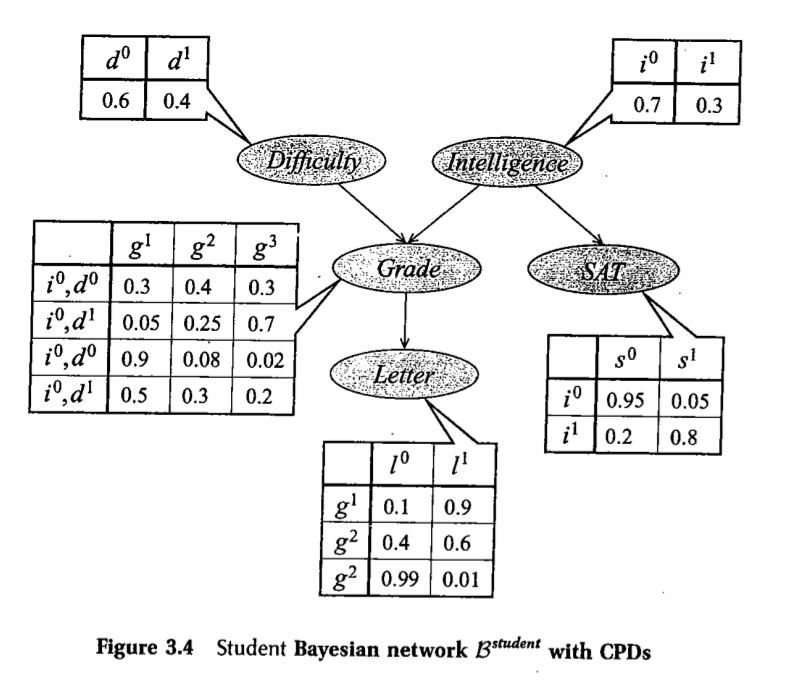
\includegraphics[width=\textwidth]{media/examplebayesnet.png}

\subsection{Adapting the model}
We note that the above Bayesian model represents explicit factorization of
joint probability distribution of all the random variables.
\begin{align}
  P(I, D, G, S, L) &= P_I(I)P_D(D)P_{G|I,D}(G|I, D)P_{S|I}(S|I)P_{L|G}(L|G)
\end{align}
where each factor corresponds to a function that is defined in Figure 3.4.

Note that each function depends only on a subset of random variables, for
example, $P_I(.)$ only depends on $I$, and $P_{G|I,D}(.)$ depends only on
$G$,$I$ and $D$.

Such a factorization can be represented as something called a \emph{factor graph} (Fig~\ref{fig:fg2}).
\begin{figure}
  \centering
  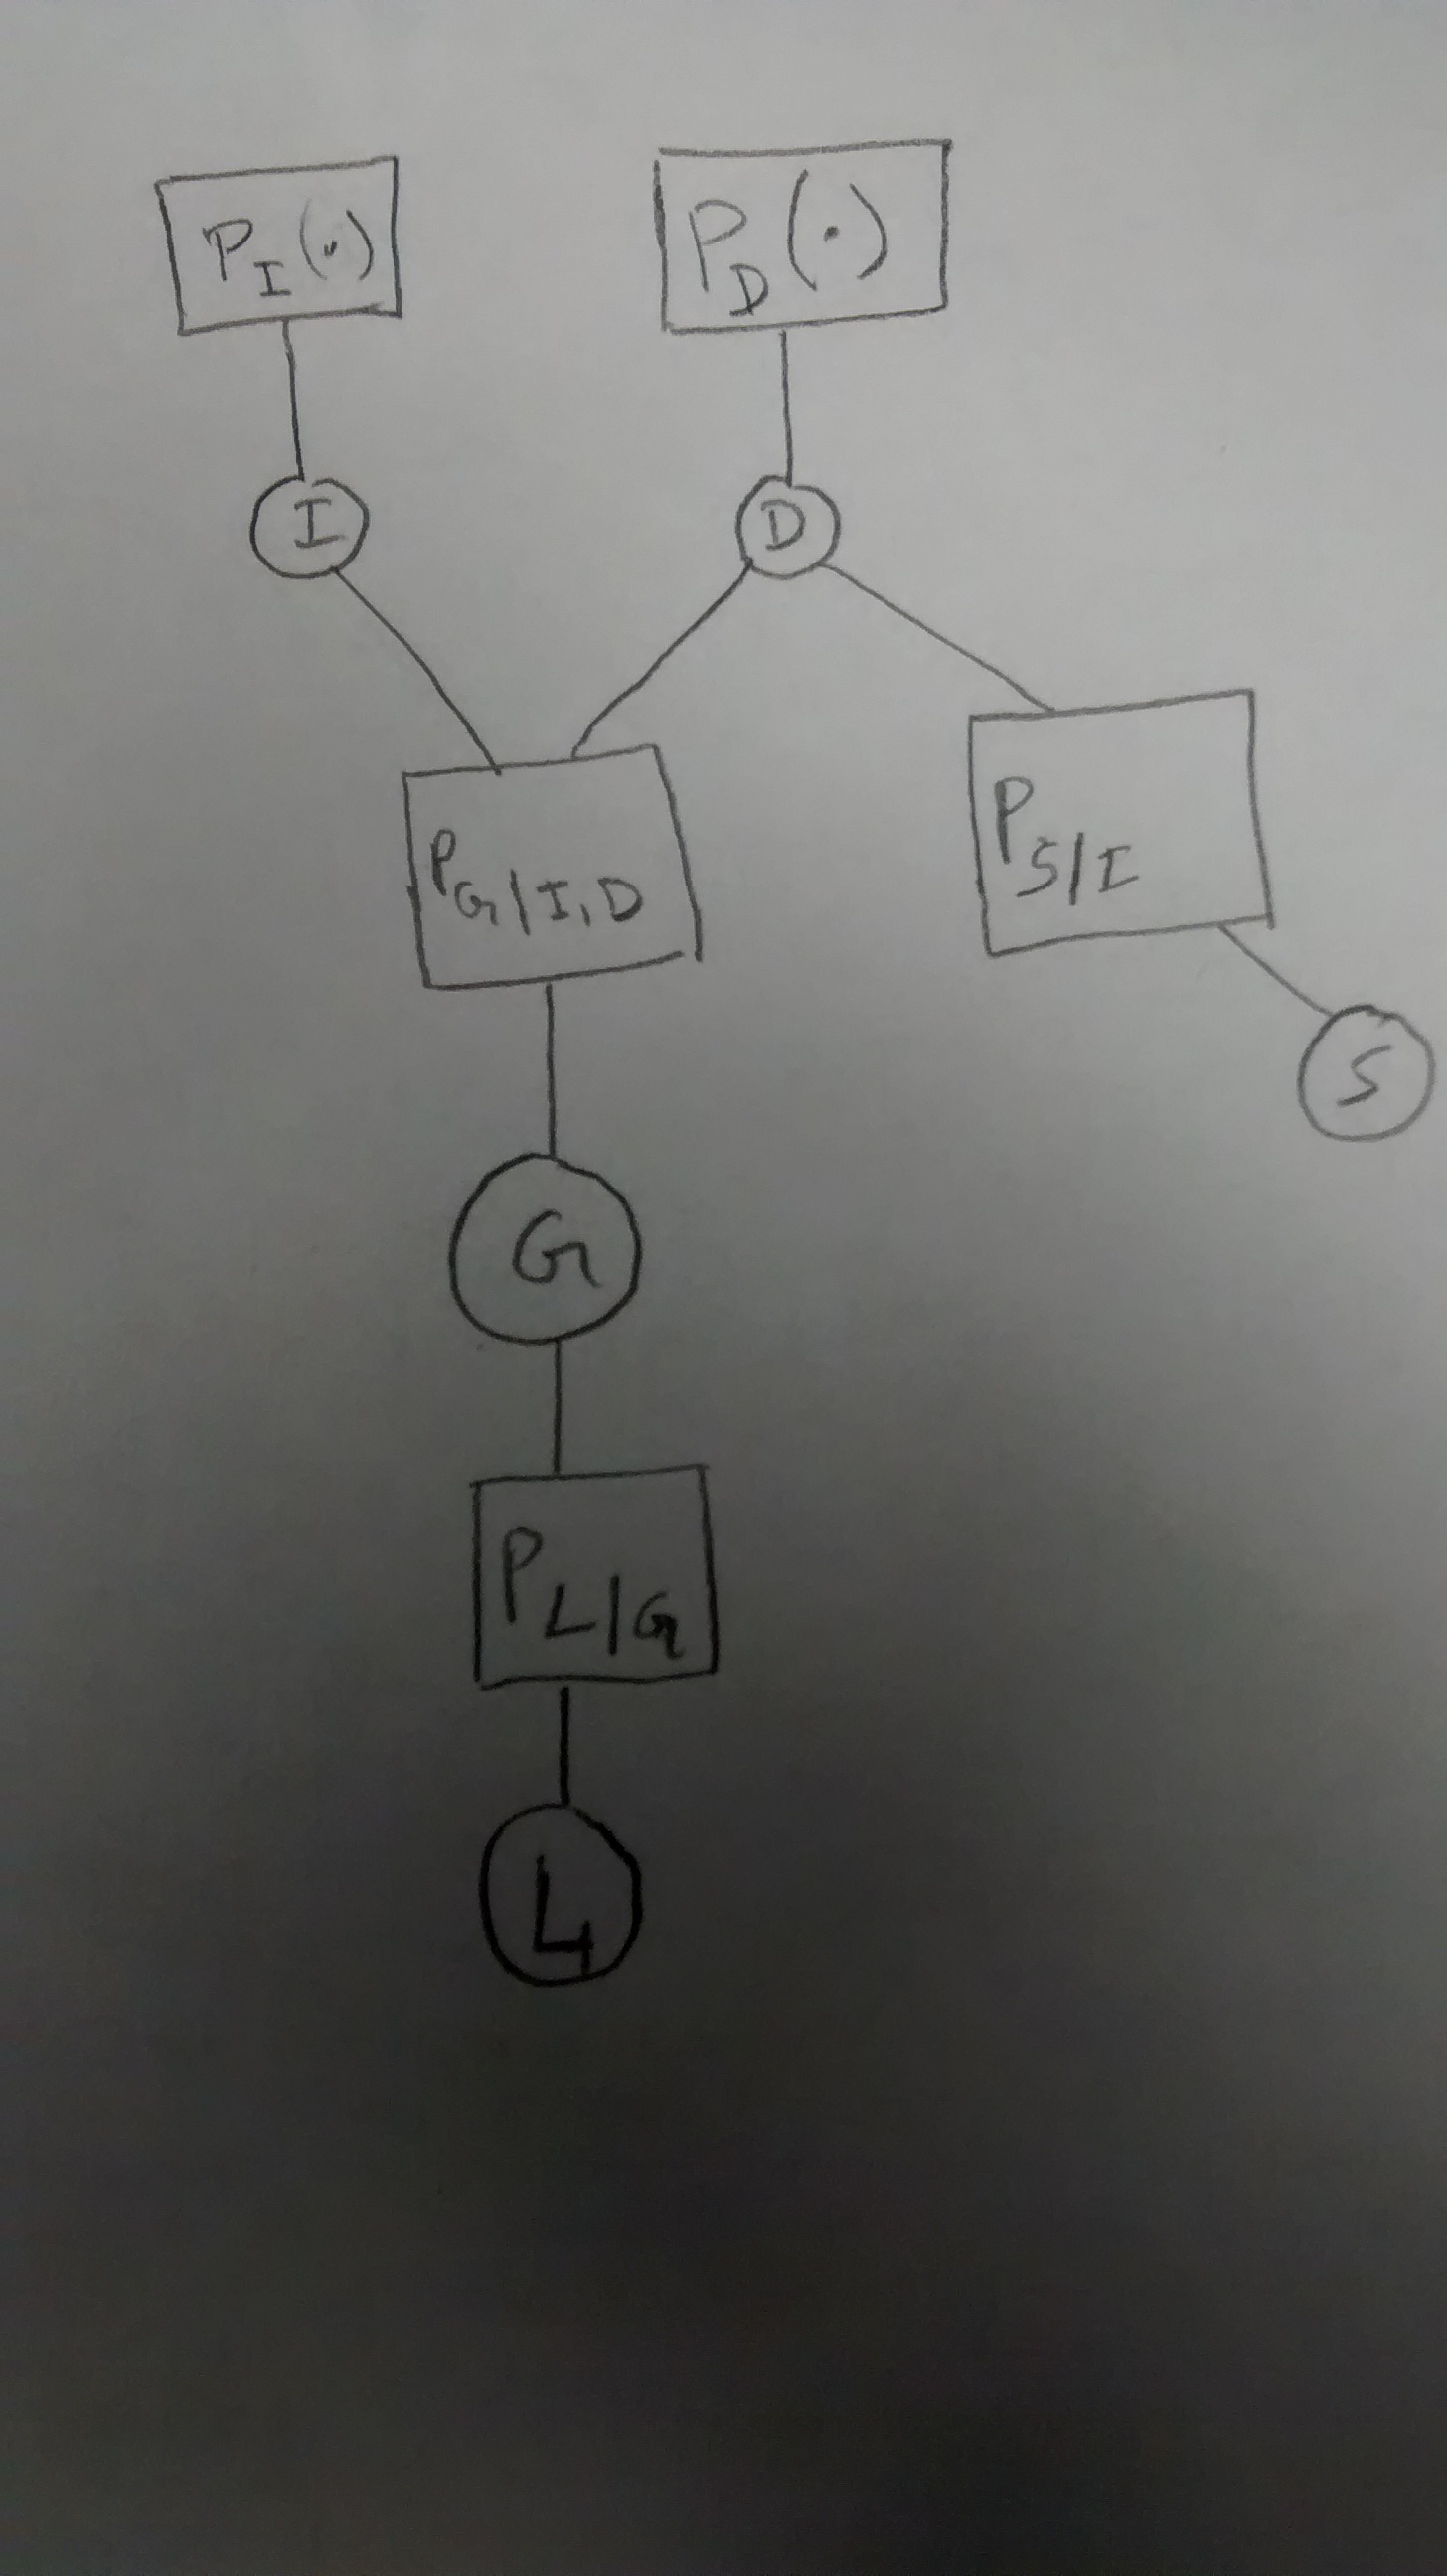
\includegraphics[height=0.58\textwidth, trim=0 8in 0 0, clip]{media/fg1.jpg}
  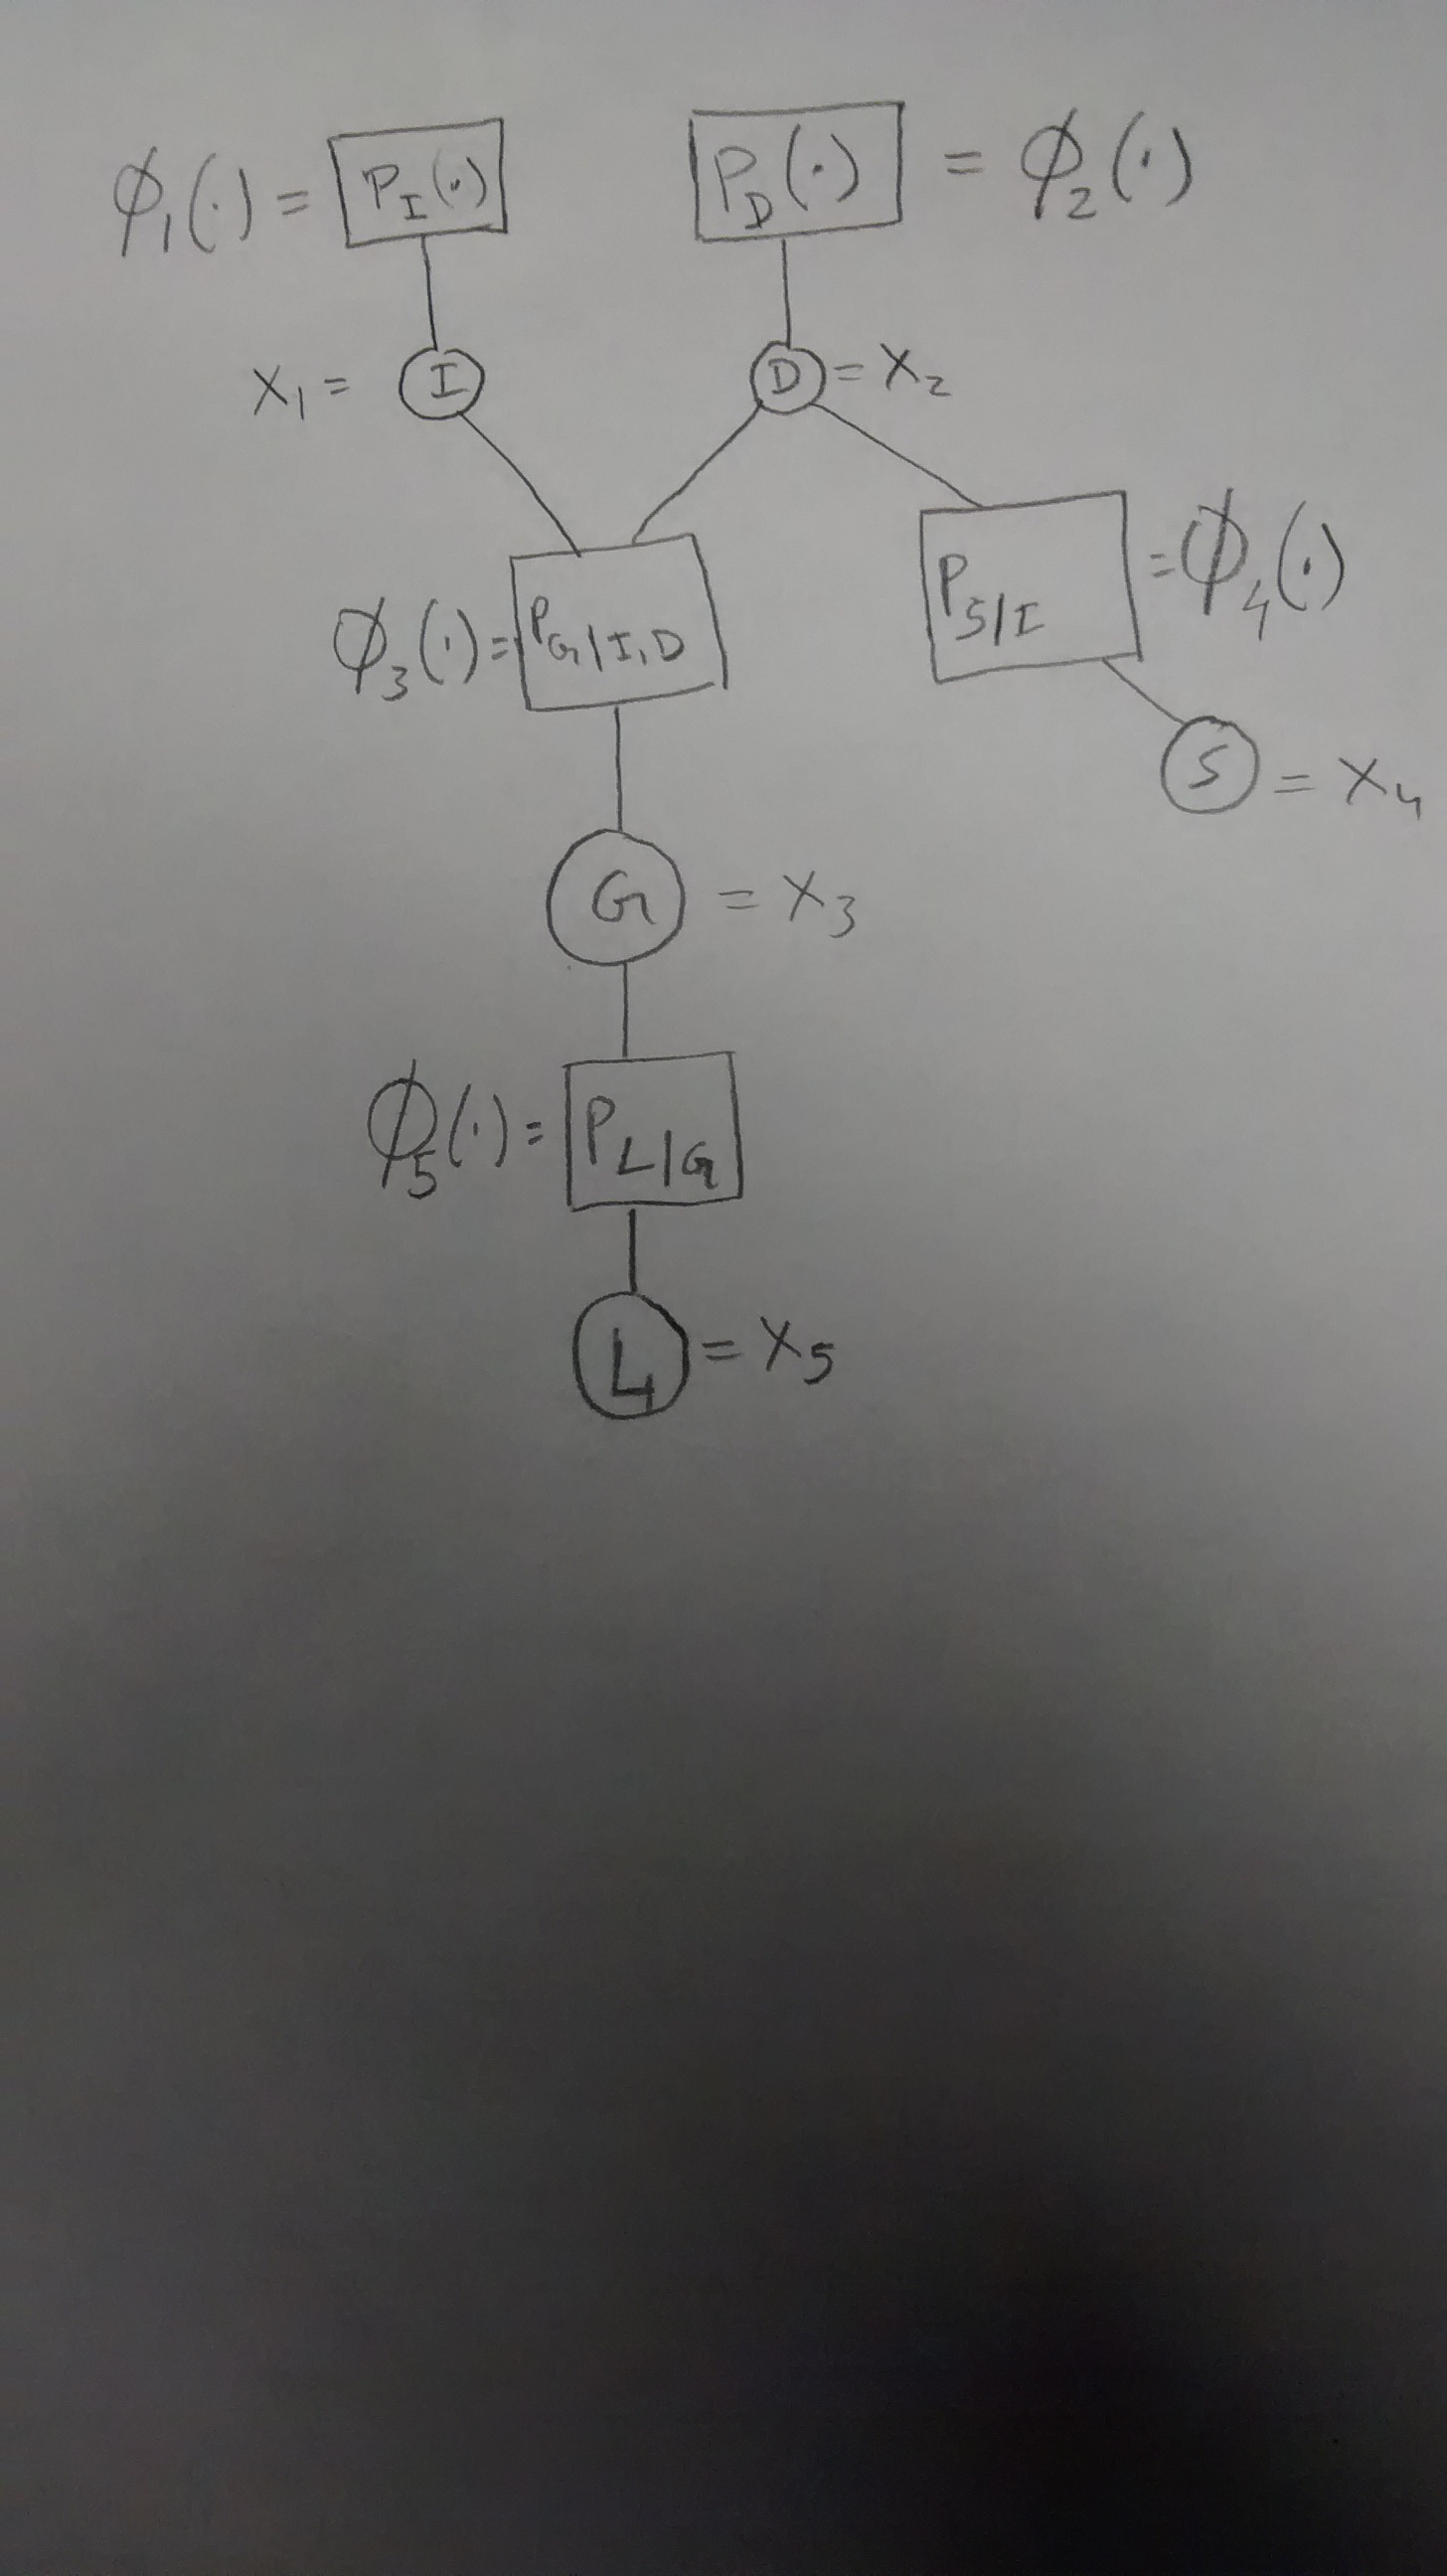
\includegraphics[height=0.58\textwidth, trim=0 15in 0 0, clip]{media/fg2.jpg}
  \caption{Factor graph representation with numbering}
  \label{fig:fg2}
\end{figure}

With this example, we are ready for a general definition of \emph{factor
graph}. 

A \emph{factor graph} is a three-tuple $(V, F, E)$ where $V$ is a set of random
variables, $F$ is a set of factors and $E$ is a set of undirected edges such
that $E = \{(X_i, \phi_j) | X_i \in V, \phi_j \in F, \phi_j \text{ depends on } X_i\}$.

\subsection{Coding the graphical model}

Modern CPP programming is a two layered programming, meta-programming (the
programming executed at compile time) and runtime-programming. 

For easier correspondence to the programmable graphical model we re-write our 
factorization in terms of $\phi_i$ and $x_i$.

\begin{align}
  P(I, D, G, S, L) &= \prod_{i=0}^{4} \phi_i(\{ x_j \}_{j : \phi_i \text{ depends on } X_j})
  \label{eq:factorization}
\end{align}

\subsubsection{Identifying the monoid}
Although the meta-programming is Turing complete, and hence we can write our
entire program in meta-programming, it is standard to use meta-programming to
deduce the types of various objects used in a CPP program.

While defining the graphical model, we have to first define the types of its
components. For this we note that all our factors $\phi_i(.)$ are of the form
$\phi_i : \{L_j\}_{j=1}^{k} \rightarrow \mathbb{R}$. It should be noted that
for a consistent graphical model, the codomain of all factors $\phi_i$ should
be consistent for valid graphical model. This codomain of all the factors is called
the \emph{ValueType}. Corresponding to the $\mathbb{R}$, we can use the CPP
datatypes like \lstinline|float| or \lstinline|double|.

Also note the operator between different factors in equation
\eqref{eq:factorization}, is multiplication. This operator acts upon the
codomain of factors $\phi_i$. The corresponding datatype in opengm is \lstinline|opengm::Multiplier|. 
Although factorization in general usage has meant with respect to multiplication, but in
abstract mathematics you can always replace one operator with another as long as it satisfies certain
axioms. Here, the operator is required to satisfy the axioms of a commutative
monoid $(\Omega, \otimes, 1)$, where $\Omega$ is the common codomain of the
factors $\phi_i$, $\otimes$ is the factorization operator and $1$ is the
identity element of the monoid such that $\forall \omega \in \Omega : \omega
\otimes 1 = \omega$. 

Note that data types/classes like \lstinline|opengm::Multiplier| and \lstinline|opengm::Adder|
corresponds to the complete monoid instead of the operator of the monoid.

The ability of using any operator in place of multiplication is of practical
importance, as it enables the use of log domain for computation without
modifying the graphical model. Log domain avoids numerical problems like
underflow and overflow.

\begin{align}
  \log P(I, D, G, S, L) &= \sum_{i=0}^{4} \log( \phi_i(\{ x_j \}_{j : \phi_i \text{ depends on } X_j}) )
  \label{eq:factorization}
\end{align}

\subsubsection{Representing the factors} 

Next step is choosing the data type for representation of factors $\phi_i(.)$.
If the corresponding function can be tabulated, then the factor can be
represented as \lstinline|opengm::ExplicitFunction|. Depending upon the structure of 
factors $\phi_i(.)$ different classes can be used. 

\begin{align}
  P_{G|I,D}(g, i, d) &= P_{G|I,D}(x_2, x_0, x_1) \\
                     &= \phi_2(x_2, x_0, x_1)
\end{align}

From the table of figure 3.4 we can explicitly assign the values for $\phi_2$

\begin{lstlisting}
  #include <opengm/functions/explicit_function.hxx>

  // Size of value space of each random variable i.e. X2, X0, X1
  size t shape[] = {3, 2, 2};
  opengm::ExplicitFunction<double> phi2(shape, shape + 3, 0.0);
  phi2(0, 0, 0) = 0.3;  phi2(1, 0, 0) = 0.4;  phi2(2, 0, 0) = 0.3;
  phi2(0, 0, 1) = 0.05; phi2(1, 0, 1) = 0.25; phi2(2, 0, 1) = 0.7;
  phi2(0, 1, 0) = 0.9;  phi2(1, 1, 0) = 0.08; phi2(2, 1, 0) = 0.02;
  phi2(0, 1, 1) = 0.5;  phi2(1, 1, 1) = 0.3;  phi2(2, 1, 1) = 0.2;
\end{lstlisting}


\subsubsection{Representing the variables}

In this course we will be dealing with discrete spaces. The general datatype to
define discrete spaces is \lstinline|opengm::DiscreteSpace|. To define and
understand this we need to tabulate the variables involved in the graphical
model and their value (or label) spaces.

\begin{tabular}{|l|l|l|r|}
  \hline
  Random Variable & Original notation & Value space & Size of Value space \\
  \hline
  $X_0$ & D & $\{d^0, d^1\}$ & 2\\
  $X_1$ & I & $\{i^0, i^1\}$ & 2\\
  $X_2$ & G & $\{g^0, g^1, g^2\}$ & 3\\
  $X_3$ & S & $\{s^0, s^1\}$ & 2\\
  $X_4$ & L & $\{l^0, l^1\}$ & 2\\
  \hline
\end{tabular}

Our representation does not requires or allows special value spaces like
$\{d^0, d^1\}$ or $\{i^0, i^1\}$ for different random variables. 
Instead all discrete value spaces are completely defined by the size of label
space. If the size of label space is $L$, then the random variable can take
values from $\{0, 1, \dots, L - 1\}$.

Hence a discrete space can be simply be defined as 

\begin{lstlisting}
  #include <opengm/graphicalmodel/space/discretespace.hxx>

  opengm::DiscreteSpace<> space;
  space.addVariable(2); // X0
  space.addVariable(2); // X1
  space.addVariable(3); // X2
  space.addVariable(2); // X3
  space.addVariable(2); // X4
\end{lstlisting}

\subsubsection{Composing the graph}

\begin{lstlisting}
  typedef opengm::GraphicalModel<MyValueType, MyOperationType, opengm::ExplicitFunction<MyValueType>, opengm::DiscreteSpace<> > GMType;
  GMType gm(space);
  typedef GMType::FunctionIndentifier GMFunctionIndentifier;
  GMFunctionIndentifier fid0 = gm.addFunction(phi0);
  GMFunctionIndentifier fid1 = gm.addFunction(phi1);
  GMFunctionIndentifier fid2 = gm.addFunction(phi2);
  GMFunctionIndentifier fid3 = gm.addFunction(phi3);
  GMFunctionIndentifier fid4 = gm.addFunction(phi4);

  gm.addFactor(fid0, var0, var0 + 1);
  gm.addFactor(fid1, var1, var1 + 1);
  gm.addFactor(fid2, var2, var2 + 3);
  gm.addFactor(fid3, var3, var3 + 2);
  gm.addFactor(fid4, var4, var4 + 2);
\end{lstlisting}

Note that we have not differentiated between factor and function in our
discussion. OpenGM does differentiate between factor and function. The distinction arises
when we can reuse certain functions. For example, if we had
$P_{L|G}(\mathbf{x}) = P_{S|I}(\mathbf{x}) \forall \mathbf{x}$, then we could
have represented both the factors with a same function.

\subsection{Adapting the problem.}
Suppose we want to find out the probability of Letter being $l^1$ given SAT score is $s^0$. Mathematically, the 

\section{Generalization}

\end{document}
